% from template https://www.overleaf.com/latex/templates/thesis-presentation-slides-unibg/kdckrhdgbqyv
\documentclass{beamer}
%\hypersetup{pdfpagemode=FullScreen} %full screen mode
\setbeamertemplate{navigation symbols}{}


\usepackage[italian]{babel} 
\usepackage[utf8]{inputenc} 
\usepackage{amsmath,amssymb}
\usepackage[T1]{fontenc} 
\usepackage{curves}
\usepackage{verbatim}
\usepackage{multimedia}
\usepackage{mathptmx}
\usepackage{graphicx}
\usepackage{booktabs}
\usepackage{hyperref}
\usepackage{multirow}
\usepackage{xcolor}
\usepackage{subcaption}
\usepackage{algorithm,algorithmic}
\usepackage{listings}

\usepackage{pgfplots}
\usepackage{amsmath}
\pgfplotsset{compat=1.18}

\lstset{
    language=Matlab,       
    basicstyle=\ttfamily\footnotesize,
    keywordstyle=\color{blue}, 
    commentstyle=\color{green},
    stringstyle=\color{red},    
    numbers=left,            
    numberstyle=\tiny,             
    numbersep=5pt,            
    breaklines=true,        
    showstringspaces=false
}

\graphicspath{{../immagini/}}

\renewcommand{\algorithmicrequire}{\textbf{Input:}}
\renewcommand{\algorithmicensure}{\textbf{Output:}}
\usepackage{lipsum}
\setbeamertemplate{caption}[numbered] % For numbering figures

\mode<presentation> {

\usetheme{Madrid} 

\usecolortheme{whale} 

%\setbeamertemplate{footline} % To remove the footer line in all slides uncomment this line


\setbeamertemplate{navigation symbols}{} % To remove the navigation symbols from the bottom of all slides uncomment this line
}

\usepackage{graphicx}
\usepackage{booktabs} 
\usepackage{dirtytalk}
\setbeamercovered{invisible}
\setbeamertemplate{bibliography item}[text]
\setbeamertemplate{theorems}[numbered]
\setbeamerfont{title}{size=\Large}%\miniscule,command,tiny, scriptsize,footnotesize,small,normalsize,large,Large,LARGE,huge,Huge,HUGE
\setbeamerfont{date}{size=\tiny}%{\fontsize{40}{48} \selectfont Text}

\setbeamertemplate{itemize items}[ball] % if you want a ball
\setbeamertemplate{itemize subitem}[circle] % if you want a circle
\setbeamertemplate{itemize subsubitem}[triangle] % if you want a triangle

%-------customized frame-------
\newcounter{cont}

\makeatletter
%allowframebreaks numbering in the title
\setbeamertemplate{frametitle continuation}{%
   % \setcounter{cont}{\beamer@endpageofframe}%
    %\addtocounter{cont}{1}%
   % \addtocounter{cont}{-\beamer@startpageofframe}%
   % (\insertcontinuationcount/\arabic{cont})%
}
\makeatother

%--------------------------
%	TITLE PAGE
%--------------------------
% electric generation and load models
\title[Photovoltaic and Load Models]{Modelli di produzione fotovoltaica e di domanda elettrica residenziale e industriale}

\author[Giulio Presti]{\texorpdfstring{{\normalsize Giulio Presti}}{Author}}

\institute[526947] %matricola
{
{\footnotesize Relatore}\\
{\footnotesize Prof. Giuseppe de Nicolao}\\
\smallskip
{\footnotesize Correlatore}\\
{\footnotesize Dott. Marco Capelletti}\\
\vspace{2.1cm}
\medskip
Dipartimento di Ingegneria Informatica e dell'Informazione\\
Università di Pavia% Your institution for the title page

%\medskip
%\textit{john@smith.com} % Your email address
}
%This will place the image at position "30 right/left and 120 up/down" relative to the top left corner of the current page.
\titlegraphic{%
  \begin{picture}(0,0)
    \put(37,128){\makebox(0,0)[rt]{
\includegraphics[width=2.30cm]{general/logo_unipv_cut.png}}}
  \end{picture}
}
 \date{30/04/2025}
 
\begin{document}
\definecolor{your_color}{HTML}{172642}
\setbeamercolor{structure}{fg=your_color}
\setbeamertemplate{footline}[page number]
\begin{frame}
\titlepage % Print the title page as the first slide


\end{frame}
\setbeamertemplate{footline}[page number]

%-------------------------------
%	PRESENTATION SLIDES
%-------------------------------

% Slide 2
\section{dataset1} 
\begin{frame}
	\frametitle{Dataset (I)}
	\vfill
	\textbf{AIMMS-MOPTA 2024 Competition}
	\vspace{0.3cm}
	\begin{itemize}
	    \item Modeling and Optimization: Theory and Applications Conference
	    \vspace{0.15cm}
	    \item Lehigh University (USA)
	    \vspace{0.15cm}
	    \item \say{Would a Fully Renewable Energy Grid benefit from adding Green Hydrogen as a Supplemental Power Source?}
	\end{itemize}
	\vfill
	\centering
	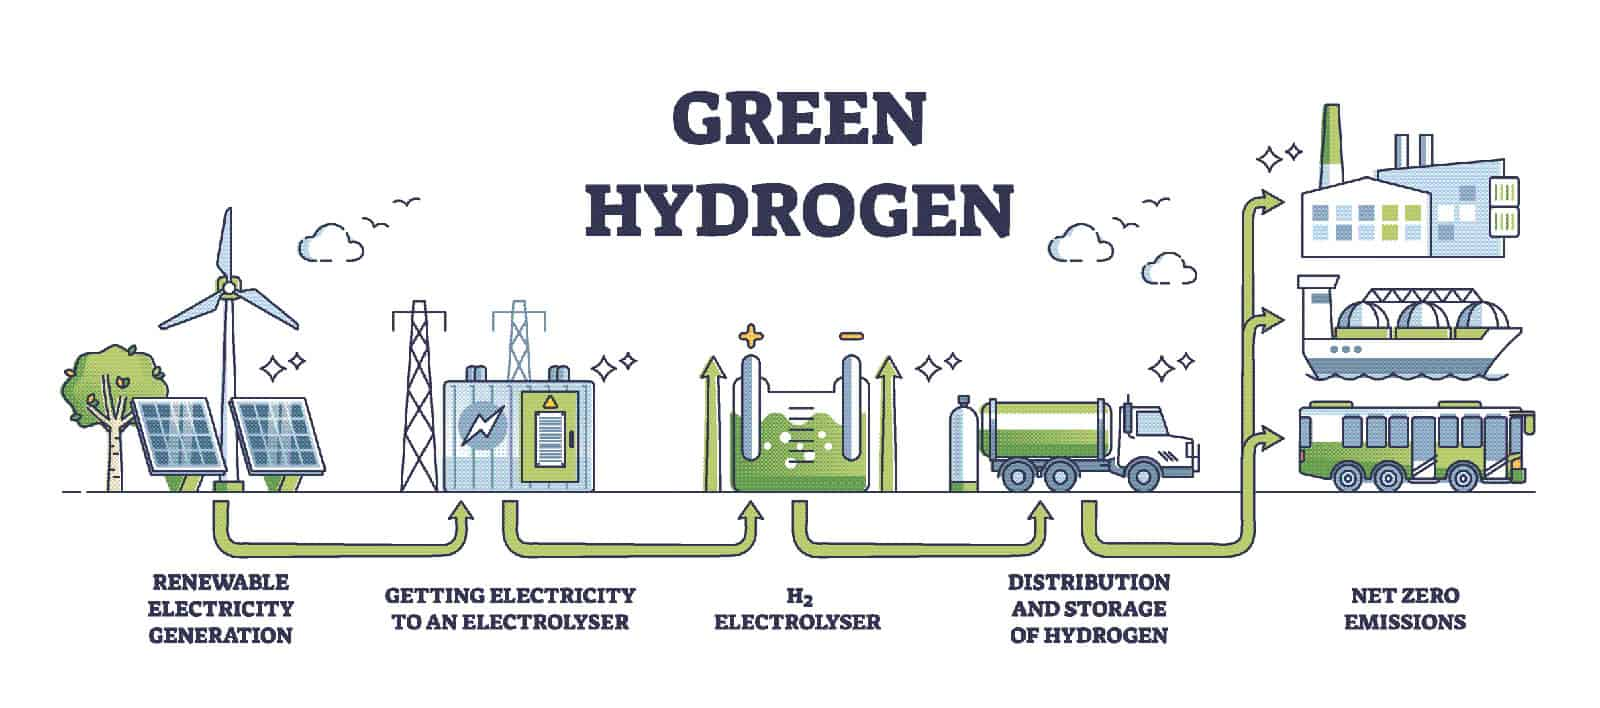
\includegraphics[width=0.8\textwidth,keepaspectratio]{general/mopta-overview.jpg}
\end{frame}

% Slide 3
\section{dataset2}
\begin{frame}
    \frametitle{Dataset (II) - Produzione fotovoltaica}
    \vfill
    
    \begin{itemize}
        \item Totale campioni: 384 (Generation) \begin{itemize}   
            \item Quarter: 4 giornate
            \item Instance: 96 rilevamenti (15 m)
        \end{itemize}
    \end{itemize}
    \vfill
    \centering
    \only<1>{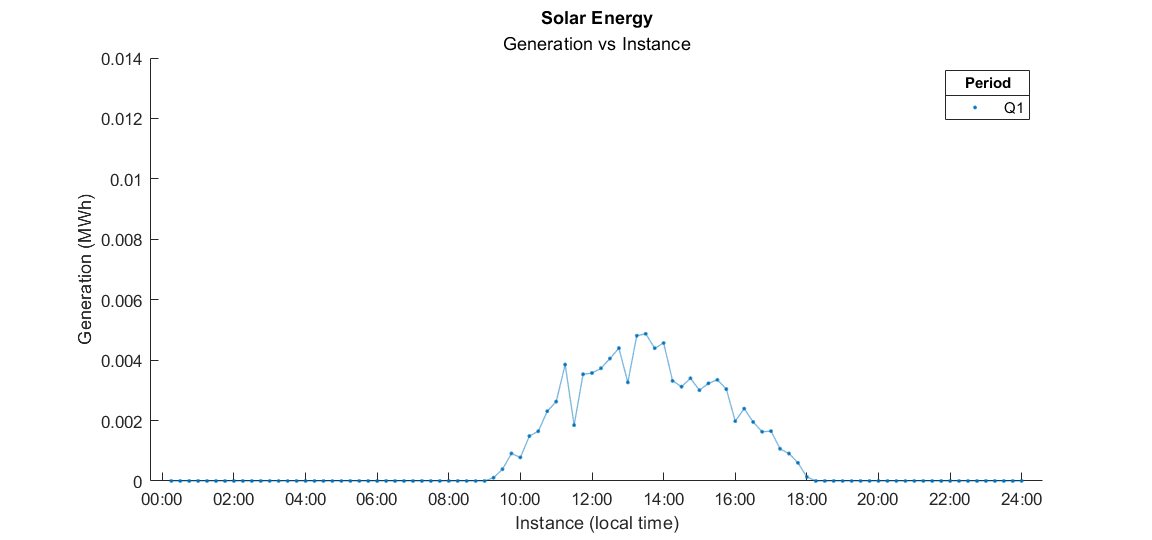
\includegraphics[width=0.9\textwidth,keepaspectratio]{solar/all_by_period_1.png}}
    \only<2>{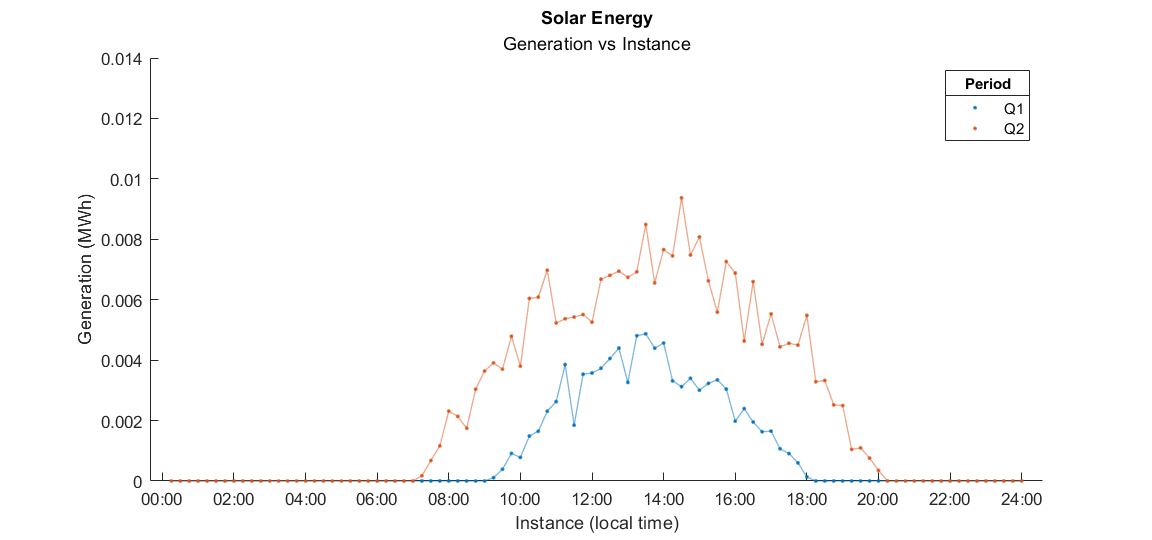
\includegraphics[width=0.9\textwidth,keepaspectratio]{solar/all_by_period_12.png}}
    \only<3>{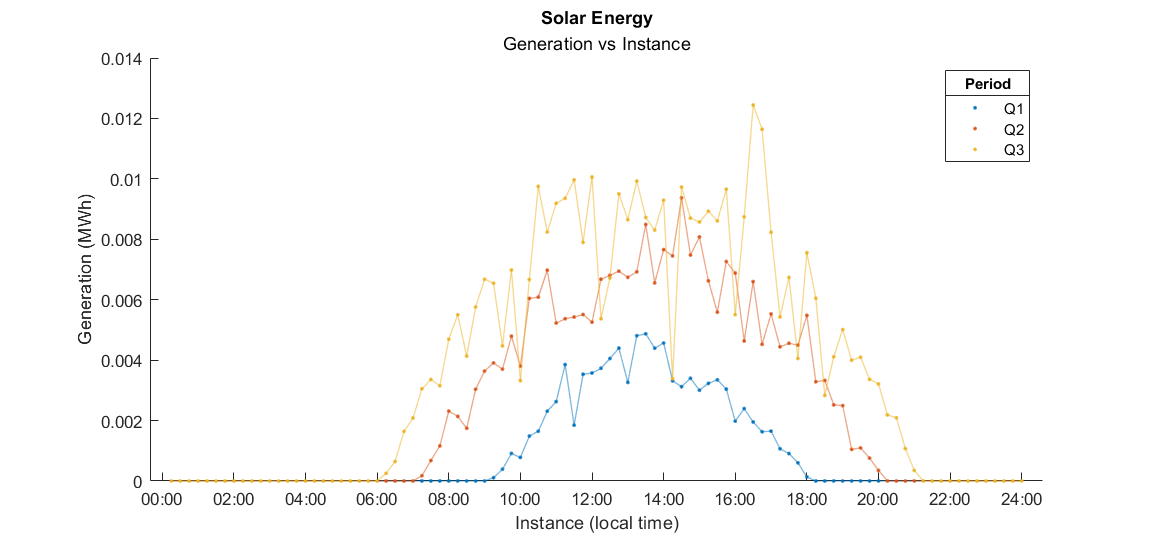
\includegraphics[width=0.9\textwidth,keepaspectratio]{solar/all_by_period_123.png}}
    \only<4>{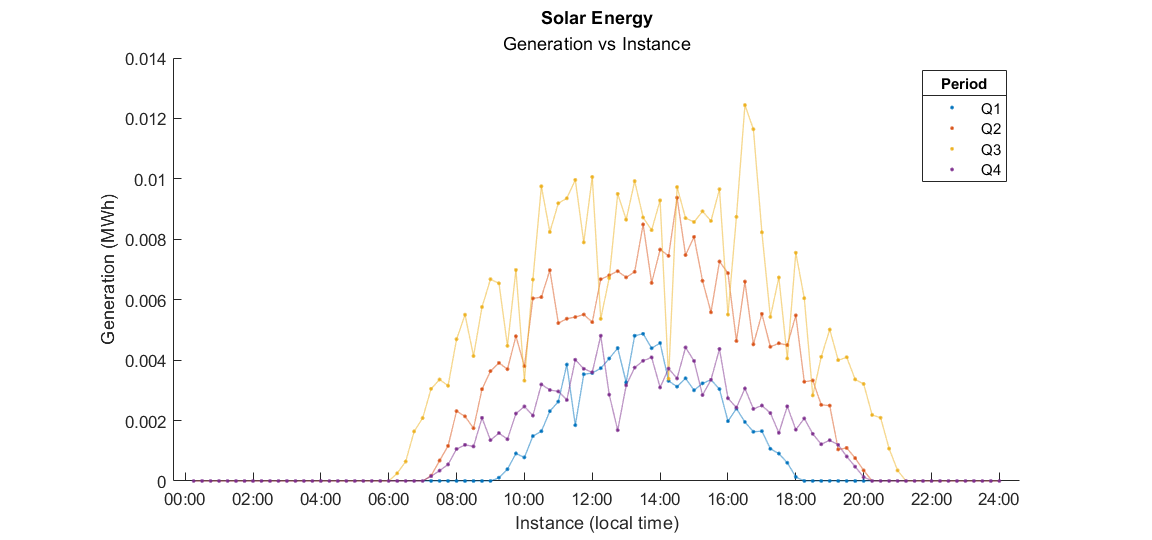
\includegraphics[width=0.9\textwidth,keepaspectratio]{solar/all_by_period_1234.png}}
        
\end{frame}

% Slide 4
\section{dataset3}
\begin{frame}
    \frametitle{Dataset (III) - Consumi elettrici}
    \vfill
    
    \begin{itemize}
        \item Totale campioni: 2688 (Load) \begin{itemize}   
            \item Quarter: 4 giornate
            \item Location: 7 posizioni
            \item Instance: 96 rilevamenti (15 m)
        \end{itemize}
    \end{itemize}
    \vfill
    \centering
    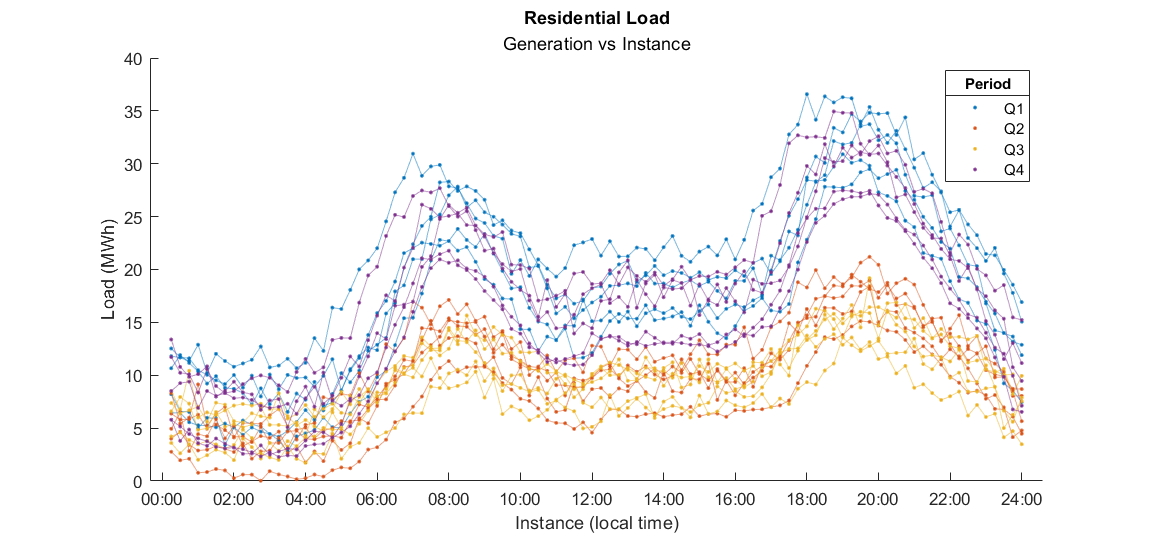
\includegraphics[width=0.9\textwidth,keepaspectratio]{all_residenzial_load_period_lines.png}
        
\end{frame}

\section{dataset3-1}
\begin{frame}
    \frametitle{Dataset (III) - Consumi elettrici}
    \vfill
    
    \begin{itemize}
        \item Totale campioni: 2688 (Load) \begin{itemize}   
            \item Quarter: 4 giornate
            \item Location: 7 posizioni
            \item Instance: 96 rilevamenti (15 m)
        \end{itemize}
    \end{itemize}
    \vfill
    \centering
    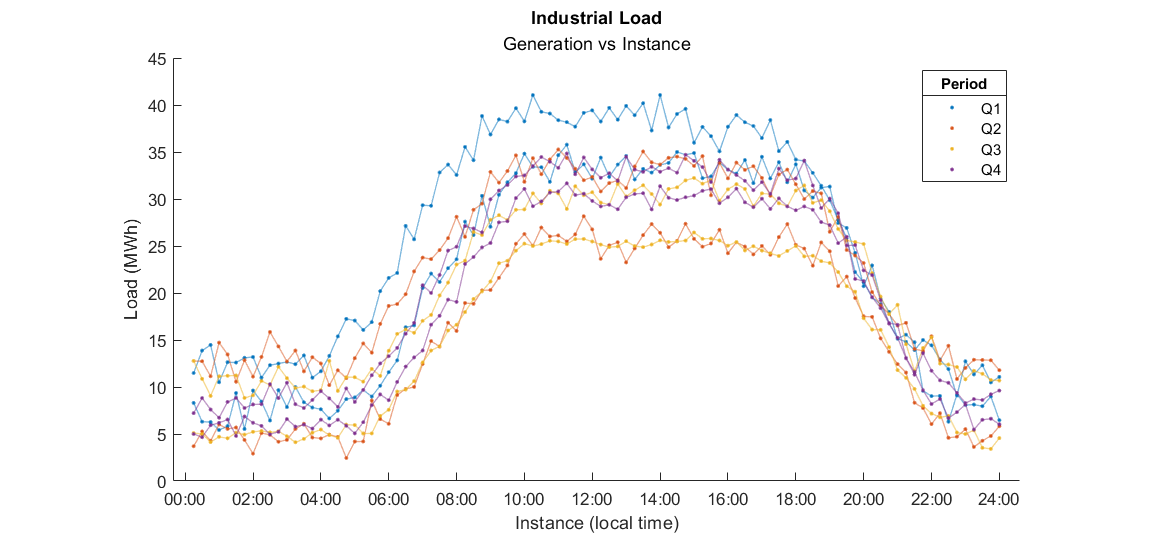
\includegraphics[width=0.9\textwidth,keepaspectratio]{all_industrial_load_period_lines.png}
        
\end{frame}

% Slide 5
\section{load-polinomial-1d}
\begin{frame}
    \frametitle{Consumi elettrici - Modelli polinomiali}
    \vfill    
    \begin{itemize}
        \item Minimi quadrati
        \item $F(x)=a_0+a_1x+a_2x^2+a_3x^3+a_4x^4...$        
        \item Scelta modello: 
            \textit{Test F}, 
            \textit{FPE}, 
            \textit{AIC}, 
            \textit{MDL}, 
            \textit{Crossvalidazione}
    \end{itemize}
    \vfill
    \centering
    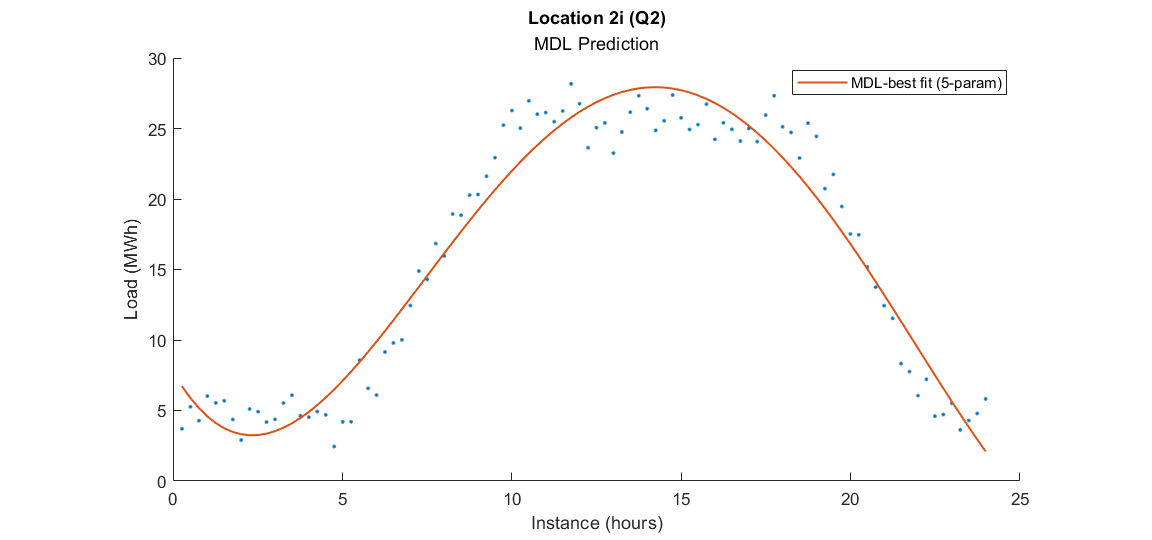
\includegraphics[width=0.9\textwidth,keepaspectratio]{2_i_q2_MDL_poli.png}     

    \scriptsize \text{5 parametri}, $MSE=5.47\text{MWh}^2$ e $R^2=0.95$
\end{frame}

\section{load-polinomial-1d-1}
\begin{frame}
    \frametitle{Consumi elettrici - Modelli polinomiali}
    \vfill    
    \begin{itemize}
        \item Minimi quadrati
        \item $F(x)=a_0+a_1x+a_2x^2+a_3x^3+a_4x^4...$        
        \item Scelta modello: 
            \textit{Test F}, 
            \textit{FPE}, 
            \textit{AIC}, 
            \textit{MDL}, 
            \textit{Crossvalidazione}
    \end{itemize}
    \vfill
    \centering
    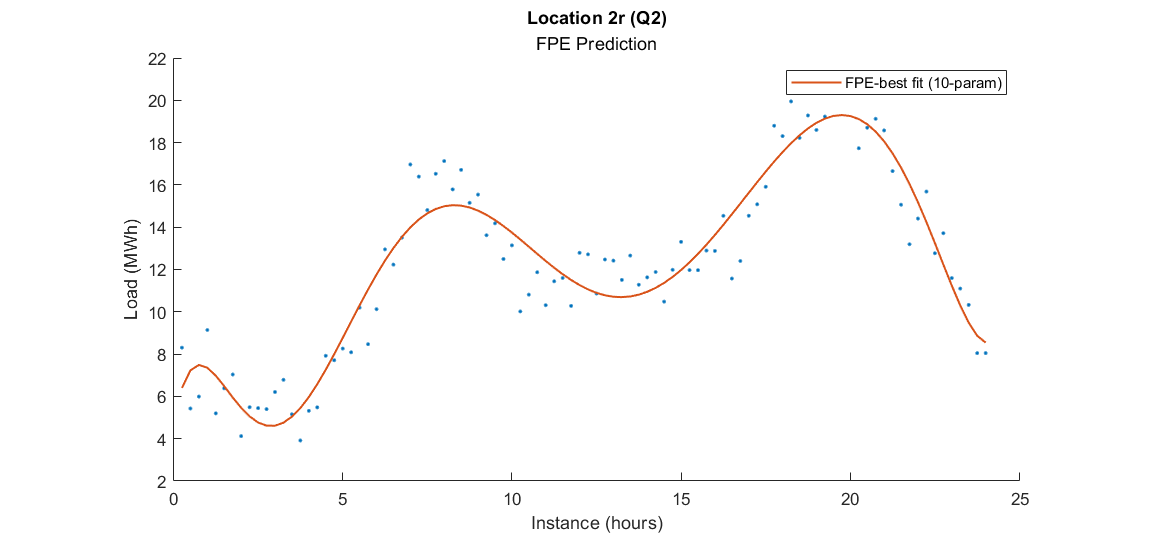
\includegraphics[width=0.9\textwidth,keepaspectratio]{2_r_q2_FPE_poli.png} 
    
    \scriptsize  \text{10 parametri}, $MSE=1.80\text{MWh}^2$ e $R^2=0.90$
\end{frame}

% Slide 6
\section{load-fourier-1d-1}
\begin{frame}
    \frametitle{Consumi elettrici - Serie di Fuorier}  
    \begin{itemize}
        \item $F(x)=b_0+
	b_1sin\left(\dfrac{2\pi}{T}x\right)+b_2cos\left(\dfrac{2\pi}{T}x\right)+...+
	b_{2k-1}sin\left(k\dfrac{2\pi}{T}x\right)+b_{2k}cos\left(k\dfrac{2\pi}{T}x\right)$    
 
    \end{itemize}
    \vfill
    \centering
    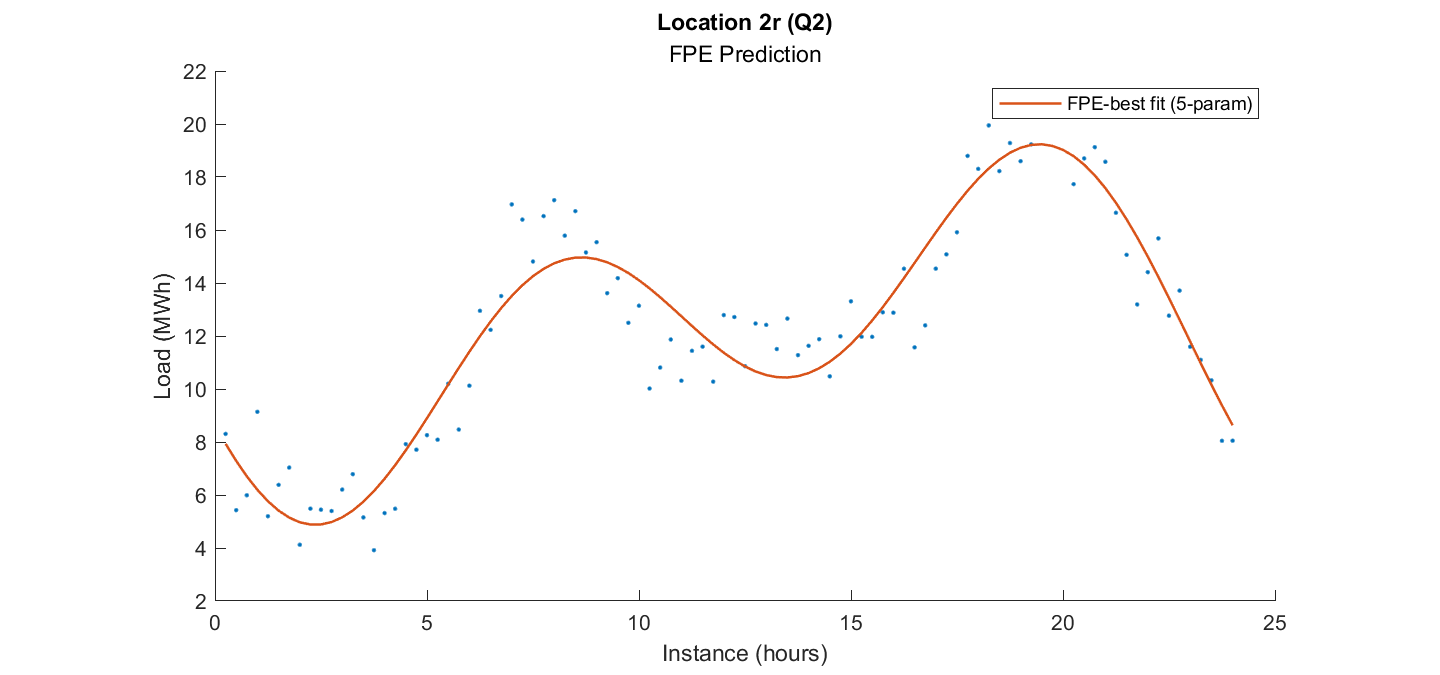
\includegraphics[width=0.9\textwidth,keepaspectratio]{2_r_q2_FPE_fourier.png} 
    
    \scriptsize  \text{5 parametri}, $MSE=2.01\text{MWh}^2$ e $R^2=0.89$
\end{frame}

\section{load-1d-summary}
\begin{frame}
    \frametitle{Consumi elettrici - Serie di Fuorier}   
    \begin{itemize}
        \item $F(x)=b_0+
	b_1sin\left(\dfrac{2\pi}{T}x\right)+b_2cos\left(\dfrac{2\pi}{T}x\right)+...+
	b_{2k-1}sin\left(k\dfrac{2\pi}{T}x\right)+b_{2k}cos\left(k\dfrac{2\pi}{T}x\right)$  
        \vspace{0.7cm}
        \item Confronto performance e flessibilità \textit{polinomi} vs \textit{serie di Fourier}: \\
        \vspace{0.3cm}
        \begin{tabular}{|c|c|c|c|c|}
            \hline
            \textbf{Location} & \textbf{Quarter} & \textbf{Model} & \textbf{N-params (FPE)} & \textbf{$R^2$} \\
            \hline
             i1 &    Q1 &    Fourier &     13 &     0.9907 \\
             i2 &     Q2 &    Poli &      5 &     0.9464 \\
             r1 &    Q3 &     Fourier &      5 &     0.8752 \\
             r2 &     Q2 &     Poli &      10 &     0.9035 \\
            \hline
        \end{tabular}
    \end{itemize}
    \vfill
\end{frame}

% Slide 7
\section{load-fourier-3d}
\begin{frame}
    \frametitle{Consumi elettrici - Modelli additivi 2D}   
    \begin{itemize}
        \item Modello in \textit{Instance} (hours) e \textit{Quarter} (days)
        \item $F(h, d)=F_i(h)+c(d)$
    \end{itemize}
    \vspace{1cm} % leave space for the next bullet
    \vfill
    
    \centering
    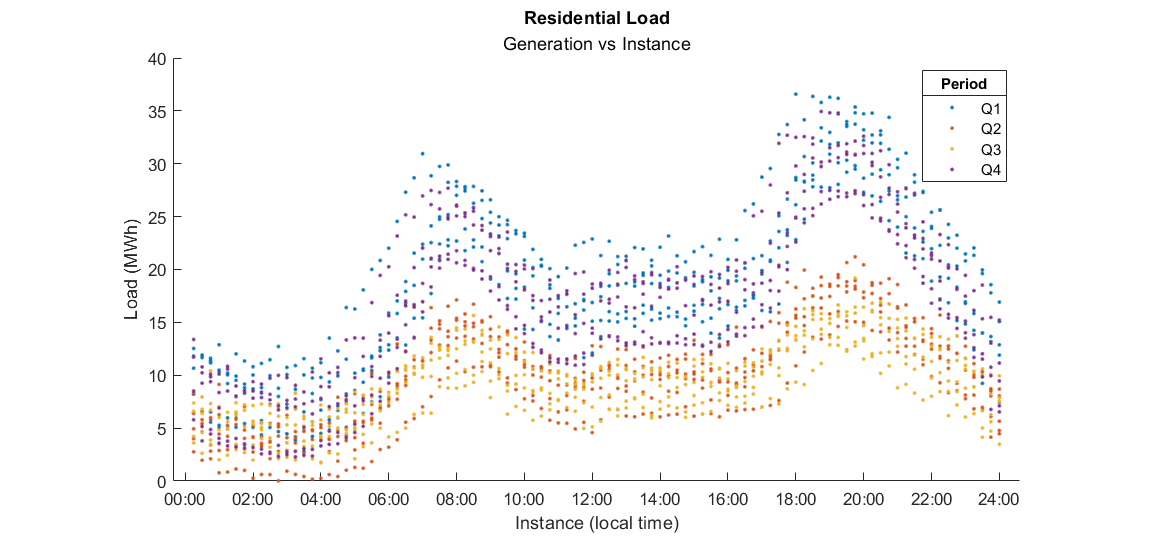
\includegraphics[width=0.9\textwidth,keepaspectratio]{all_residenzial_load_period.png} 
\end{frame}

\section{load-fourier-3d-1}
\begin{frame}
    \frametitle{Consumi elettrici - Modelli additivi 2D}   
    \begin{itemize}
        \item Modello in \textit{Instance} (hours) e \textit{Quarter} (days)
        \item $F(h, d)=F_i(h)+c(d)$
        \item $c(d)$ di tipo polinomiale o periodico
    \end{itemize}
    \vfill
    \centering
    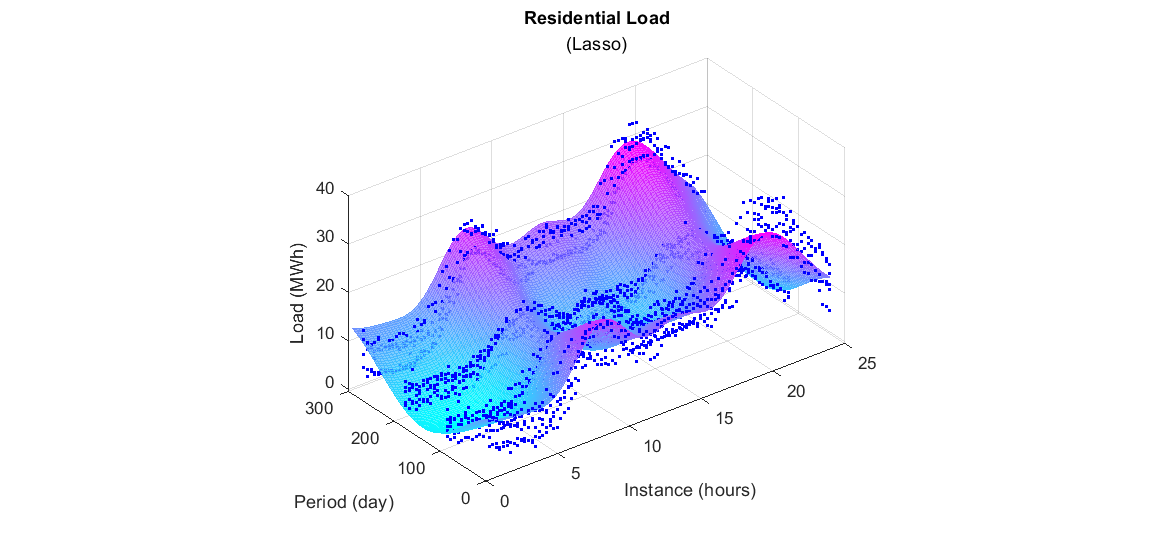
\includegraphics[width=0.9\textwidth,keepaspectratio]{all_residential_load_lasso_const_f.png} 
    
    \scriptsize  \text{12 parametri}, $MSE=10.2\text{MWh}^2$ e $R^2=0.81$
\end{frame}

\section{load-fourier-3d-2}
\begin{frame}
    \frametitle{Consumi elettrici - Modelli additivi 2D}   
    \begin{itemize}
        \item Modello in \textit{Instance} (hours) e \textit{Quarter} (days)
        \item $F(h, d)=F_i(h)+c(d)$
        \item $c(d)$ di tipo polinomiale o periodico
    \end{itemize}
    \vspace{0.3cm}
    \vfill
    \centering
    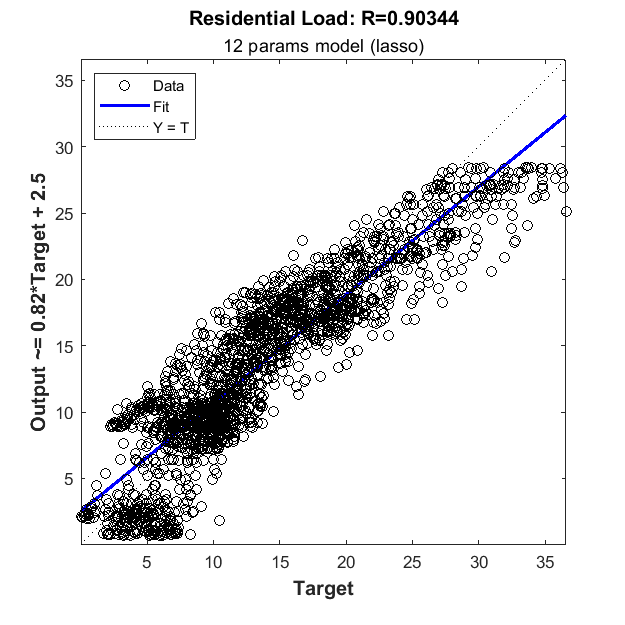
\includegraphics[width=0.42\textwidth,keepaspectratio]{all_residential_load_lasso_const_f_plotregression.png} 

    \scriptsize \text{12 parametri}, $MSE= 10.2\text{MWh}^2$ e $R^2=0.82$
\end{frame}

\section{load-fourier-3d-3}
\begin{frame}
    \frametitle{Consumi elettrici - Modelli additivi 2D}   
    \begin{itemize}
        \item Modello in \textit{Instance} (hours) e \textit{Quarter} (days)
        \item $F(h, d)=F_i(h)+c(d)$
        \item $c(d)$ di tipo polinomiale o periodico
    \end{itemize}
    \vspace{0.3cm}
    \vfill
    \centering
    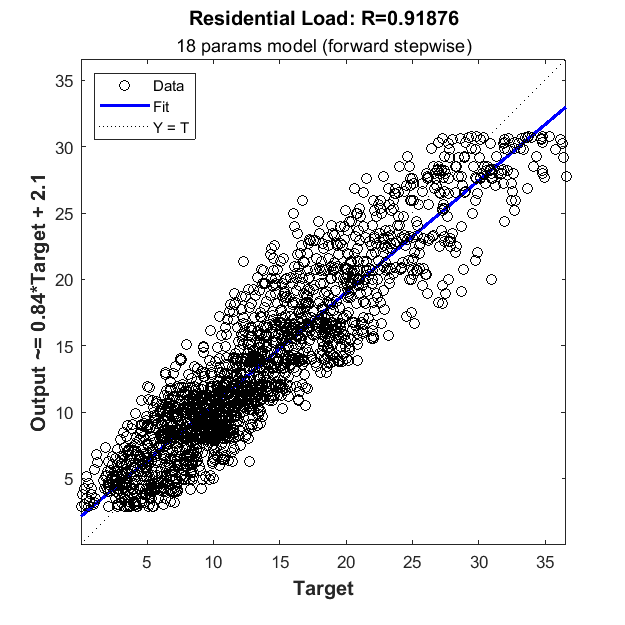
\includegraphics[width=0.42\textwidth,keepaspectratio]{all_residential_load_forw_plotregression.png} 

    \scriptsize \text{18 parametri}, $MSE= 8.72\text{MWh}^2$ e $R^2=0.84$
\end{frame}

% Slide 8
\section{solar-fourier-3d-3}
\begin{frame}
    \frametitle{Generazione solare - Modelli 2D}   
    \begin{itemize}
        \item<1-> Una sola Location
        \item<2-> Problematiche di derivabilità
        \item<3-> Feature selection:
        \textit{Lasso}, 
        \textit{Forward stepwise}, 
        \textit{Backward stepwise}
    \end{itemize}
    
    \begin{overlayarea}{\textwidth}{\textheight}
        \vfill
        \centering
        \only<1>{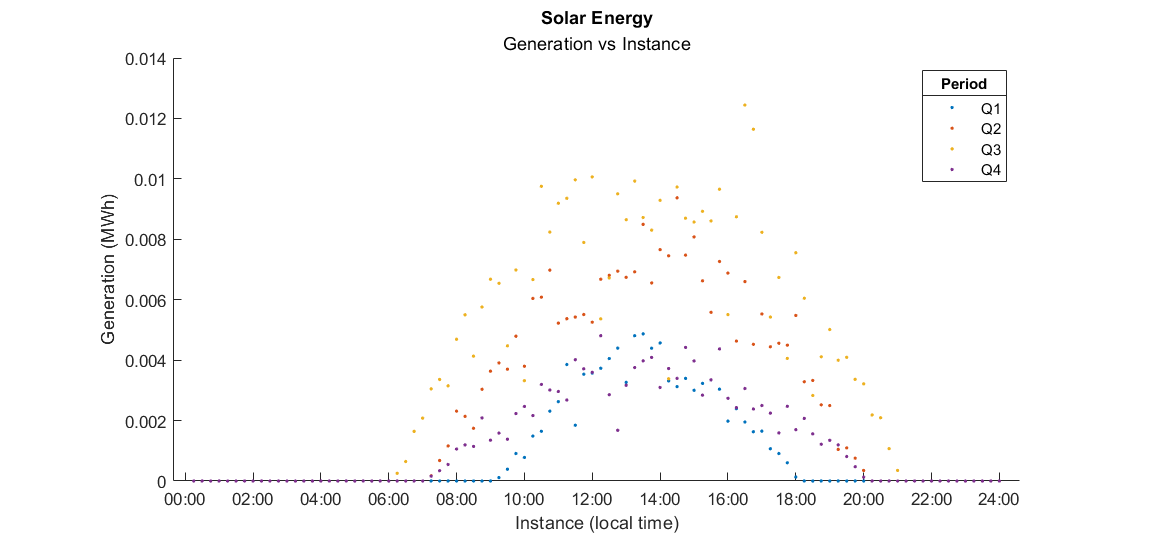
\includegraphics[width=0.9\textwidth]{solar/all_by_period.png}}
        \only<2>{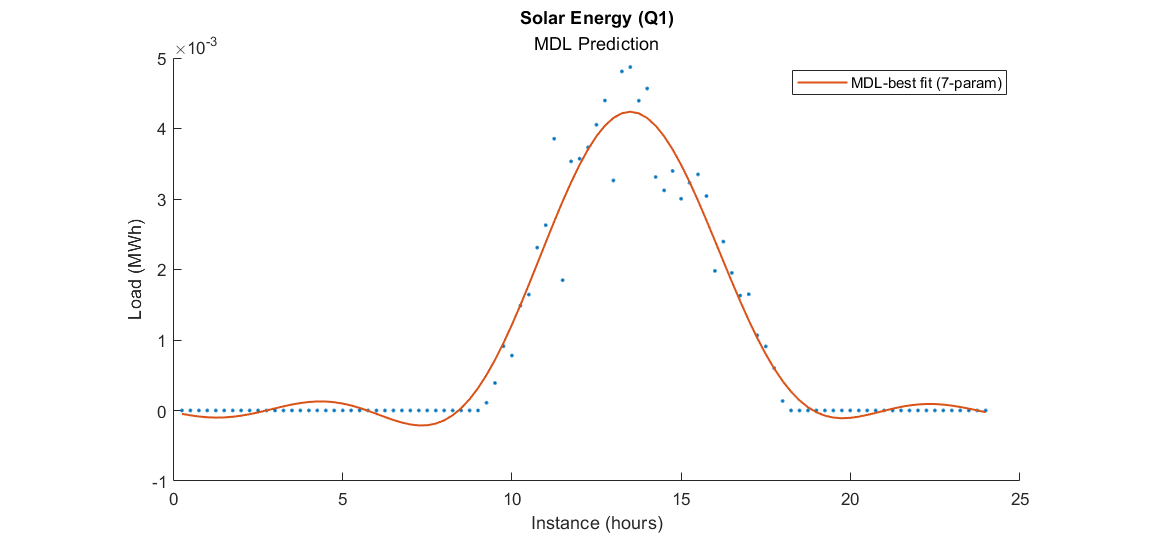
\includegraphics[width=0.9\textwidth]{solar/q1_MDL_fourier.png}}
        \only<3>{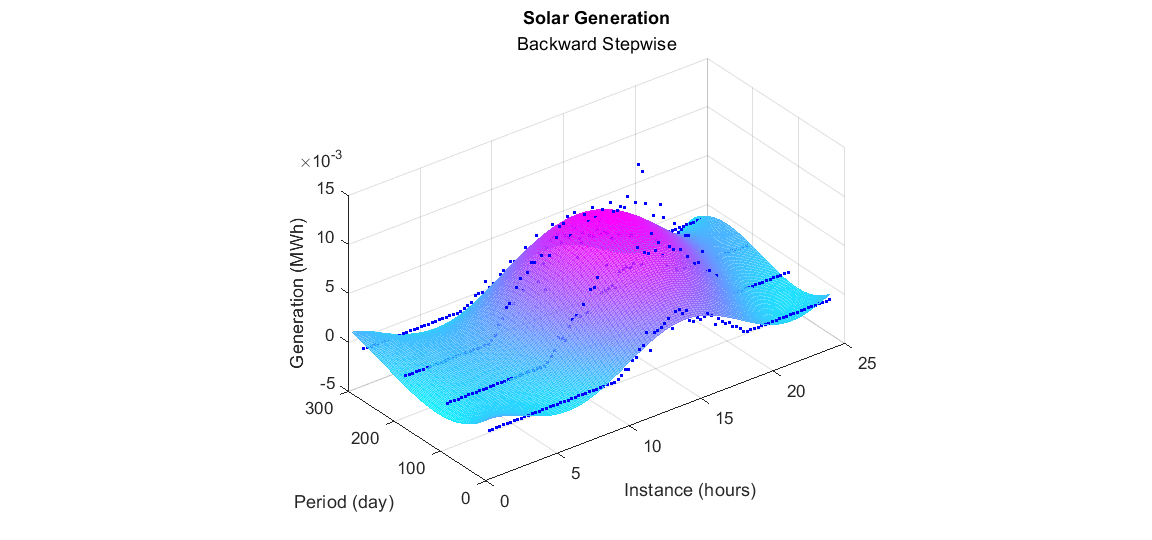
\includegraphics[width=0.9\textwidth]{solar/all_3d_poli_backward.png}}
        \only<3>{\scriptsize \text{15 parametri}, $MSE= 9.43\cdot 10^{-7}\text{MWh}^2$ e $R^2=0.89$}
    \end{overlayarea}
\end{frame}

% Slide 9
\section{solar-fourier-positive}
\begin{frame}
    \frametitle{Generazione solare - Generazione positiva}   
    \begin{itemize}
        \item $\{G | G(h, d)>0\}$
        \vspace{0.2cm}
        \item Teorema di Gauss-Markov\begin{itemize}
             \vspace{0.2cm}
            \item $\theta^{blue}=(\Phi^T\Psi^{-1}\Phi)^{-1}\Phi^T\Psi^{-1}Y$
        \end{itemize}
        \item $f_I(g)=k\cdot f_I(g|s)\cdot f_I(s)$
        
    \end{itemize}
    
    \begin{overlayarea}{\textwidth}{\textheight}
        \vfill
        \centering
        \only<1>{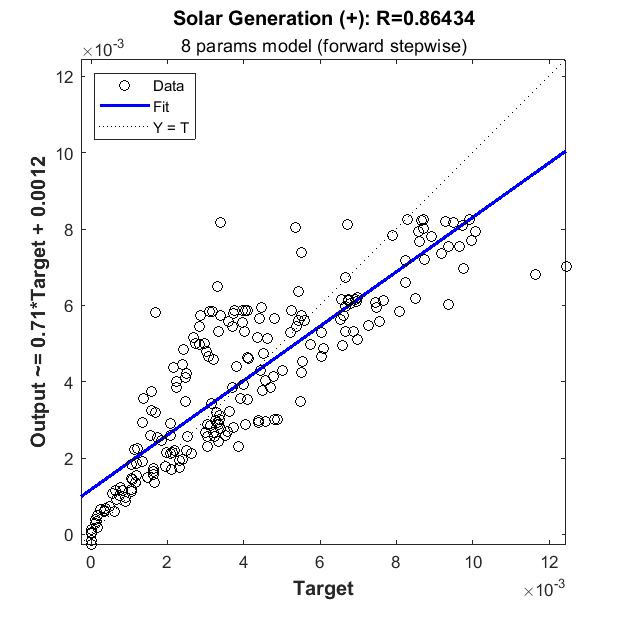
\includegraphics[width=0.4\textwidth]{solar/all_pos_poli_forward_plotregression.png}}
        \only<2>{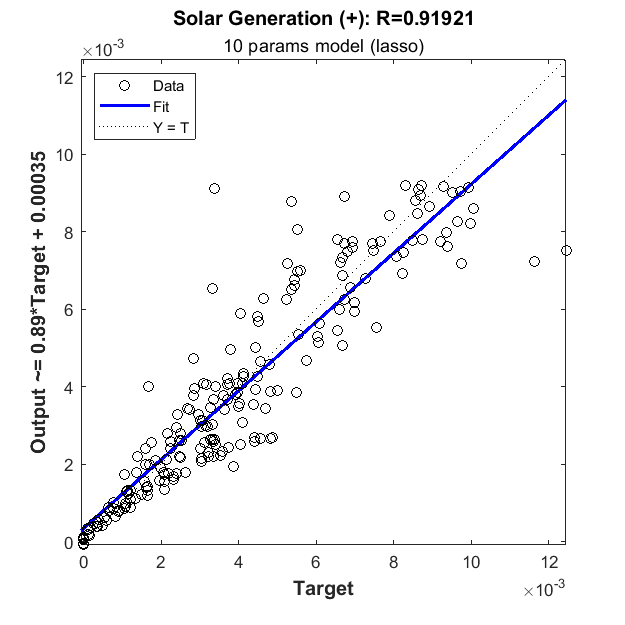
\includegraphics[width=0.4\textwidth]{solar/all_pos_fourier_forward_plotregression.png}}
        \only<3>{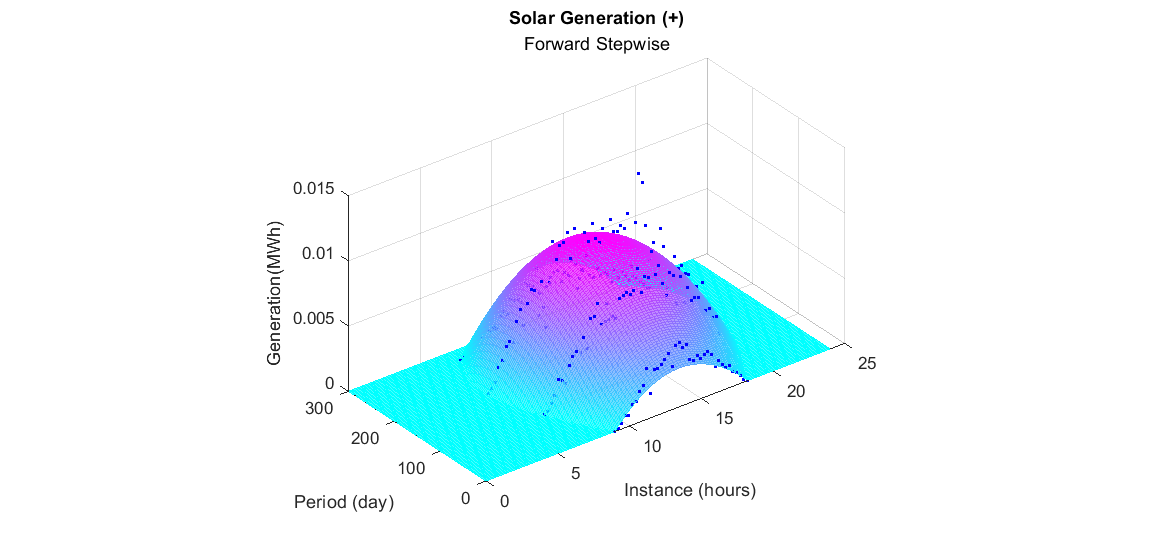
\includegraphics[width=0.9\textwidth]{solar/all_pos_poli_forward.png}}
        
        \only<1>{\scriptsize \text{8 parametri}, $MSE=2.05\cdot 10^{-6}\text{MWh}^2$ e $R^2=0.75$}
        \only<2>{\scriptsize \text{10 parametri}, $MSE=1.29\cdot 10^{-6}\text{MWh}^2$ e $R^2=0.84$}
        \only<3>{\scriptsize \text{8 parametri}, $MSE=2.05\cdot 10^{-6}\text{MWh}^2$ e $R^2=0.75$}
    \end{overlayarea}
\end{frame}

\begin{frame}
\Huge{\centerline{Grazie per l'attenzione}}
\end{frame}


\appendix
\setcounter{page}{1}
\renewcommand{\thepage}{A\arabic{page}}
\setbeamertemplate{footline}{
  \hfill
  \insertpagenumber\hspace{1em}\vspace{1em}
}


\section{appendice}

\begin{frame}[fragile]
    \frametitle{Esempio matrice di sensitività $\Phi$}
\small 
\begin{lstlisting}
Ty = 365;
Td = 24;

Phi=@(instances, periods)[
    instances.^0 ... % cost
    ... % 1 ord
    cos(1*2*pi/Td*instances) sin(1*2*pi/Td*instances)...
    cos(1*2*pi/Ty*periods) sin(1*2*pi/Ty*periods)...
    cos(1*2*pi/Td*instances).*cos(1*2*pi/Ty*periods) sin(1*2*pi/Td*instances).*cos(1*2*pi/Ty*periods)...
    cos(1*2*pi/Td*instances).*sin(1*2*pi/Ty*periods) sin(1*2*pi/Td*instances).*sin(1*2*pi/Ty*periods)...
    ... % 2 ord
    cos(2*2*pi/Td*instances) sin(2*2*pi/Td*instances)... 
    cos(2*2*pi/Ty*periods) sin(2*2*pi/Ty*periods)...
    ... % altri ordini
    ]
\end{lstlisting}
    
\end{frame}

\begin{frame}
    \frametitle{Riferimenti}

    \begin{itemize}
        \item MOPTA24 Competition Dataset, \url{https://coral.ise.lehigh.edu/~mopta2024/}.
        \vspace{0.3cm}
        \item MOPTA24 Competition Dataset, \textit{MOPTA Competition Optimization Problem}, Marco Capelletti, Luca Danna, Anna Sacilotto.
        \vspace{0.3cm}
        \item \textit{The Elements of
Statistical Learning}, Trevor Hastie, Robert Tibshirani, Jerome Friedman.
    \end{itemize}
\end{frame}

\begin{frame}
    \frametitle{Load Quarter - Problemi}
    \begin{itemize}
        \item \say{This demand data can be considered indicative of a typical demand pattern for the region during that quarter.} (AIMMS-MOPTA 2024 - "Data")
        \item Il testo della competizione non specifica la regolarità del campionamento durante l'anno.
    \end{itemize}
    \vspace{0.5cm}
    \vfill
    \begin{overlayarea}{\textwidth}{\textheight}
        \vfill
        \centering
        \only<1>{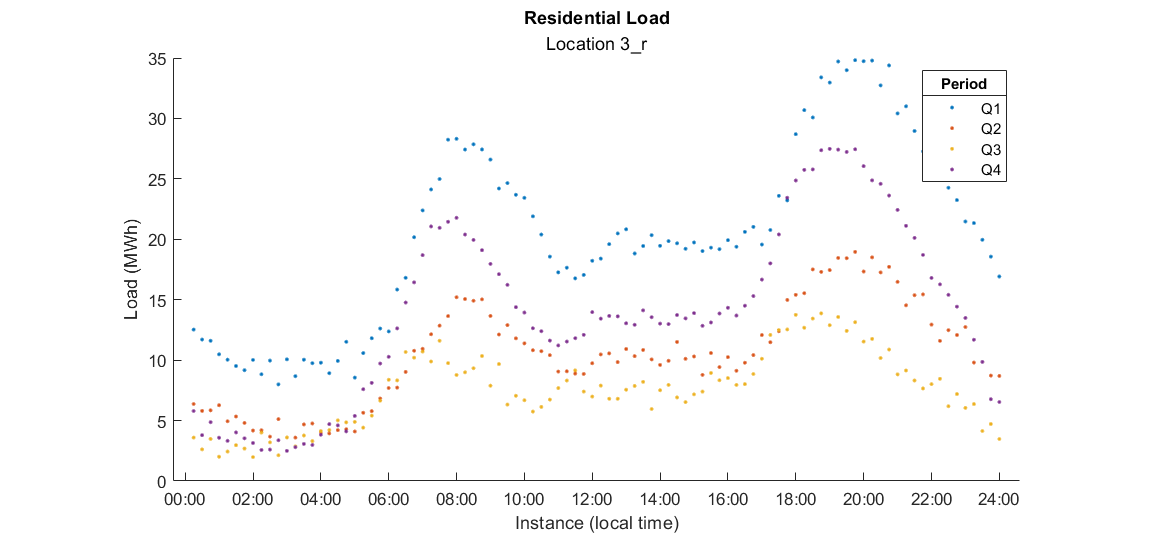
\includegraphics[width=0.9\textwidth]{3_r_load_by_period.png}}
        \only<2>{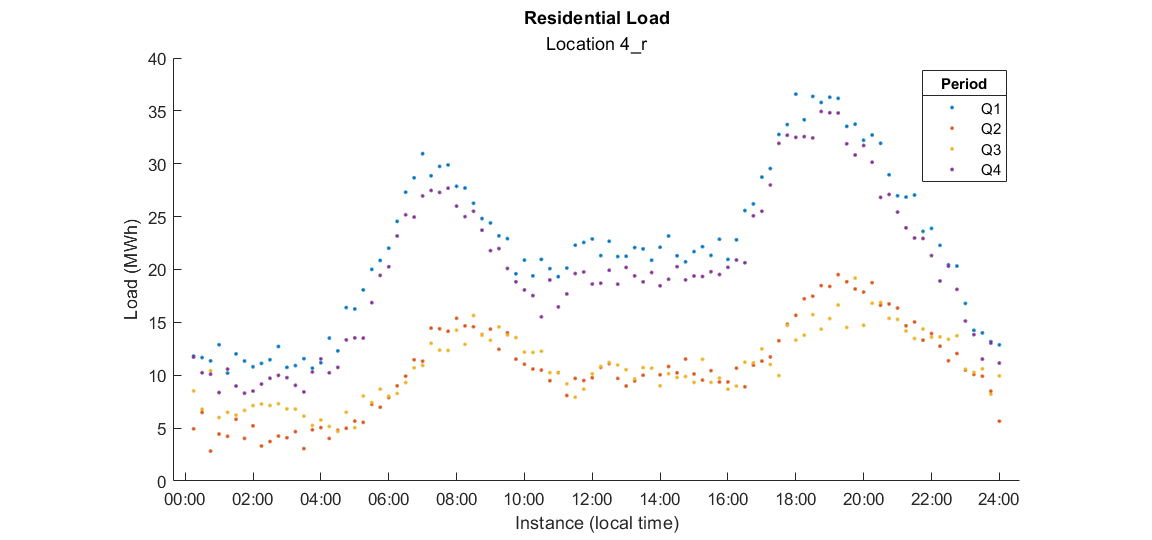
\includegraphics[width=0.9\textwidth]{4_r_load_by_period.png}}
    \end{overlayarea}
\end{frame}

\begin{frame}
    \frametitle{Blackout - Spagna}
    \begin{itemize}
        \item Poco prima che si verificasse il blackout, si è avuto un picco di produzione di energia solare.
	\item  Lunedì 28 alle 12.30
    \end{itemize}
    \vfill
    \begin{overlayarea}{\textwidth}{\textheight}
        \vfill
        \centering
        \only<1>{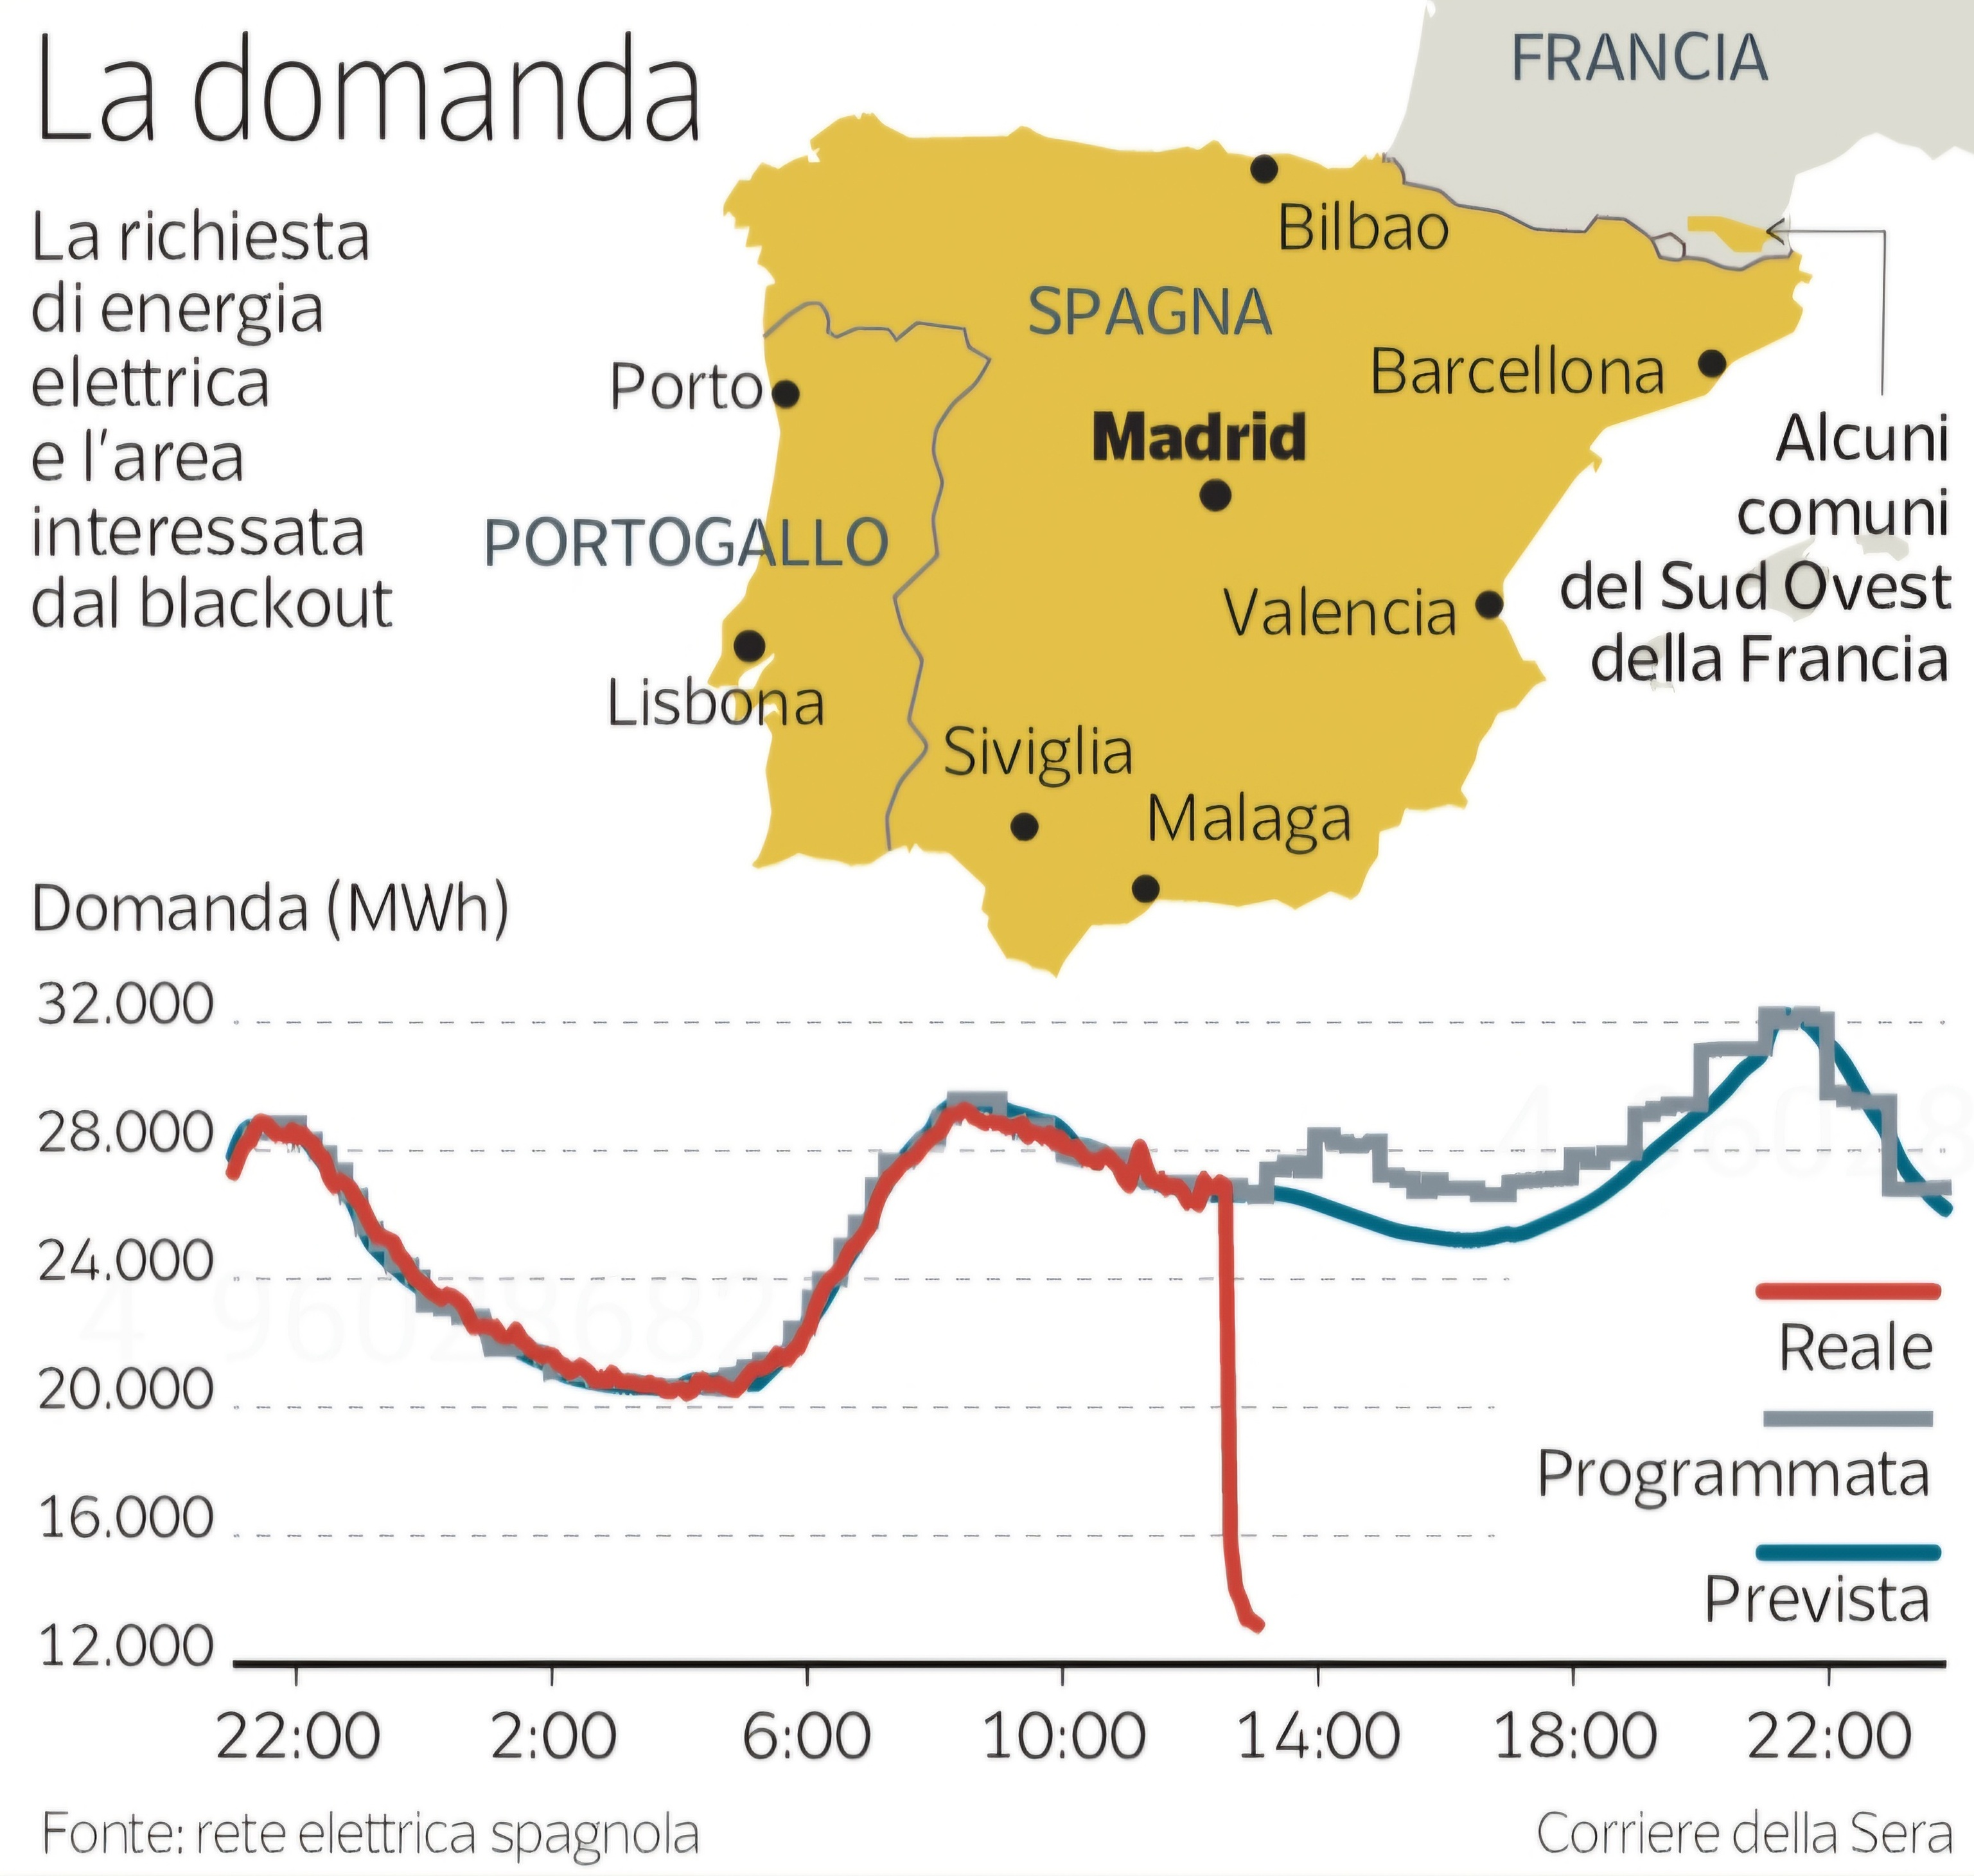
\includegraphics[width=0.55\textwidth]{general/spagna_blackout.jpg}}
    \end{overlayarea}
\end{frame}

% \begin{frame}
%     \frametitle{Aliasing (Quarter)}
%     \begin{tikzpicture}
% \begin{axis}[
%     width=12cm,
%     height=7cm,
%     xmode=log,
%     xlabel={Frequenza ($1/d$ log scale)},
%     ylabel={$c_n$},
%     xmin=0, xmax=0.15,
%     ymin=0, ymax=1.2,
%     xtick={0.00274, 0.00548, 0.14286},
%     xticklabels={$\frac{1}{365}$, $\frac{2}{365}$, $\frac{1}{7}$},
%     ytick={0, 0.2, 0.4, 0.6, 0.8, 1.0},
%     grid=both,
%     title={Andamento componenti serie di Fourier},
% ]

% % Delta in 1/365
% \addplot[
%     impulse,
%     color=blue,
%     mark=none,
%     domain=0.0027:0.0028,
%     samples=2,
%     line width=2pt
% ] coordinates {(0.00274, 0) (0.00274, 1)};

% % Delta in 2/365
% \addplot[
%     impulse,
%     color=blue,
%     mark=none,
%     domain=0.0054:0.0055,
%     samples=2,
%     line width=2pt
% ] coordinates {(0.00548, 0) (0.00548, 1)};

% % Delta in 1/7
% \addplot[
%     impulse,
%     color=blue,
%     mark=none,
%     domain=0.1428:0.1429,
%     samples=2,
%     line width=2pt
% ] coordinates {(0.14286, 0) (0.14286, 1)};

% \draw[red, dashed, line width=1.5pt] (axis cs:0.00548,0) -- (axis cs:0.00548,1.1) 
%     node[pos=1.05, align=center, font=\small];

% \end{axis}
% \end{tikzpicture}
% \end{frame}

\end{document}

